% Created 2017-01-25 Wed 18:35
% Intended LaTeX compiler: pdflatex
\documentclass[10pt,a4paper]{tufte-handout}
\usepackage{fontspec}
\usepackage{graphicx}
\usepackage{grffile}
\usepackage{longtable}
\usepackage{wrapfig}
\usepackage{rotating}
\usepackage[normalem]{ulem}
\usepackage{amsmath}
\usepackage{textcomp}
\usepackage{amssymb}
\usepackage{capt-of}
\usepackage{hyperref}
\usepackage{microtype}
\usepackage{newunicodechar}
\usepackage{unicodesymbols}
\usepackage[notions,operators,sets,keys,ff,adversary,primitives,complexity,asymptotics,lambda,landau]{cryptocode}
\usepackage{xspace}
\usepackage{units}
\usepackage{nicefrac}
\usepackage{gensymb}
\usepackage{amsthm}
\usepackage{amsmath}
\usepackage{amssymb}
\usepackage{xcolor}
\usepackage{listings}
\usepackage[color=yellow!40]{todonotes}
\newunicodechar{ }{~}
\newtheorem{lemma}{Lemma}
\newtheorem{theorem}{Theorem}
\newtheorem{definition}{Definition}
\newtheorem{remark}{Remark}
\newtheorem{corollary}{Corollary}
% LaTeX header for org-mode lab assignments. 
%
% This file assumes
%
% - the standard org-mode prefix
% - #+LATEX_CLASS: handout
% - #+LATEX_CLASS_OPTIONS: [10pt,a4paper]
% - (setq org-latex-default-packages-alist
%      (remove* '("T1" "fontenc" t) org-latex-default-packages-alist :test 'equal))

\usepackage{ifxetex}

\ifxetex
  \renewcommand{\textls}[2][5]{%
    \begingroup\addfontfeatures{LetterSpace=#1}#2\endgroup
  }
  \renewcommand{\allcapsspacing}[1]{\textls[15]{#1}}
  \renewcommand{\smallcapsspacing}[1]{\textls[10]{#1}}
  \renewcommand{\allcaps}[1]{\textls[15]{\MakeTextUppercase{#1}}}
  \renewcommand{\smallcaps}[1]{\smallcapsspacing{\scshape\MakeTextLowercase{#1}}}
  \renewcommand{\textsc}[1]{\smallcapsspacing{\textsmallcaps{#1}}}
\fi

\RequirePackage[backend=bibtex,
            style=alphabetic,
            maxnames=4,
            citestyle=alphabetic]{biblatex}

\bibliography{local.bib,abbrev3.bib,crypto_crossref.bib}

\setmonofont[BoldFont={Cousine Bold},
             ItalicFont={Cousine Italic},
             BoldItalicFont={Cousine Bold Italic},
             Scale=MatchLowercase]{Cousine}

\makeatletter
\patchcmd{\@verbatim}
  {\verbatim@font}
  {\verbatim@font\scriptsize}
  {}{}
\makeatother

\DeclareMathOperator{\Vol}{Vol}

\setlength{\parindent}{0em}
\setlength{\parskip}{1em}
\setlength{\RaggedRightParindent}{0em}

\usepackage{xcolor}
\lstset{showstringspaces=false,
        aboveskip=0.75em,
        basicstyle=\footnotesize\ttfamily,
        keywordstyle=\bfseries\color{gray!40!black},
        commentstyle=\itshape\color{gray!140!black},
        identifierstyle=\color{gray!40!black},
        stringstyle=\color{gray},
        backgroundcolor=\color{gray!190!black},
        frame=none,
        xleftmargin=\parindent}

\hypersetup{
  linkcolor=gray!40!black,
  colorlinks=true,
  citecolor=gray!40!black,
  linkcolor=gray!40!black,
  urlcolor=gray!40!black}

\author{Martin R. Albrecht and Léo Ducas}
\date{March 23, 2017}
\title{Lab 2\\\medskip
\large Attacks \& Lattice Reduction}
\hypersetup{
pdfauthor={Martin R. Albrecht and Léo Ducas},
pdftitle={Lab 2},
pdfkeywords={},
pdfsubject={},
pdfcreator={Emacs 25.1.1 (Org mode 9.0.3)},
pdflang={English},
colorlinks,
citecolor=gray,
filecolor=gray,
linkcolor=gray,
urlcolor=gray
}
\begin{document}

\maketitle
In this lab, we will make intensive use of Fplll\footnote{\url{https://github/com/fplll/fplll}} and Fpylll\footnote{\url{https://github.com/fplll/fpylll}}. Fplll is a C++11 library for operating on lattices using floating point arithmetic. It implements Gram-Schmidt orthogonalisation, LLL, BKZ, BKZ 2.0 \footfullcite{AC:CheNgu11}, Slide reduction \footfullcite{STOC:GamNgu08} and Self-Dual BKZ \footfullcite{EPRINT:MicWal15}.

Fpylll is a Python wrapper and extension of Fplll, making its data structures and algorithms available in Python and Sage (7.4 and greater). It also (re-)implements some algorithms in Python to make their internals easily accessible, a feature we will make use of.

\textbf{Note:} Both Fplll and Fpylll are evolving software projects. In particular, the current development versions of either library offer improvements over the latest stable released shipped with Sage. Thus, using Fpylll from within Sage and compiling your own version outside of Sage from GitHub will be different. We recommend, if at all possible, to use the latest development version.\footnote{You can install the latest development versions of fplll/fpylll into Sage as well, if you run Sage locally, i.e. not on \url{https://sagemath.com}}

That both libraries are evolving software projects also means that (a) you will encounter bugs and (b) we need your help. For example, you will notice that some functions lack documentation, examples and tests. Contributions welcome!\footnote{\url{https://github.com/fplll/fplll/blob/master/CONTRIBUTING.md}}

\section{1 — Introduction}
\label{sec:org33cf1d8}
In this lab, we ask you to experiment with LLL and BKZ (2.0) as implemented in Fpylll. We start with a little tutorial on how to use this library. 

To start, we first import the \texttt{fpylll} API into Sage’s main namespace:

\lstset{language=sage,label= ,caption= ,captionpos=b,numbers=none}
\begin{lstlisting}
from fpylll import *
\end{lstlisting}

\subsection{Integer Matrices}
\label{sec:org3c42bd5}

To experiment, we generate a \(q\)-ary lattice of dimension 100 and determinant \(q^{50}\) where \(q\) is a 30-bit prime. Before we sample our basis, we set the random seed to ensure we can reproduce our experiments later.

\lstset{language=sage,label= ,caption= ,captionpos=b,numbers=none}
\begin{lstlisting}
set_random_seed(1337)
A = IntegerMatrix.random(100, "qary", k=50, bits=30)
\end{lstlisting}

\textbf{Reminder:} Objects and functions in Python/Sage can be interrogated to learn more about them such as what parameters they accept (for functions) or (often) their documentation.\footnote{\url{https://doc.sagemath.org/html/en/tutorial/tour\_help.html}}

\subsection{Gram-Schmidt Orthogonalisation}
\label{sec:org354a7af}

To run LLL we have two choices. We can either run the high-level \texttt{LLL.reduction()} function or we can create the appropriate hierarchy of objects “by hand”. That is, algorithms are represented by objects with which we can interact. As this exercise is about dealing with those internal objects, we are going to pursue this strategy. We, hence, first create a \texttt{MatGSO} object, which takes care of computing the Gram-Schmidt orthogonalisation. 

A \texttt{MatGSO} object stores the following information:

\begin{itemize}
\item An integral basis \texttt{B},
\item the Gram-Schmidt coefficients \(μ_{i,j} = ⟨b_i, b^*_j⟩ / \|b^*_j\|^2\) for \(i>j\),
\item the coefficients \(r_{i,i} = ⟨b^*_i, b^*_i⟩\) and
\item the coefficients \(r_{i,j} = ⟨b_i, b^*_j⟩ = μ_{i,j} ⋅ r_{j,j}\) for \(i>j\)
\end{itemize}

It holds that: \(B = R × Q = (μ × D) × (D^{-1} × B^*)\) where \(Q\) is orthonormal, \(R\) is lower triangular and \(B^*\) is the Gram-Schmidt orthogonalisation.

We choose the floating point type (≈ bits of precision) used to represent the Gram-Schmidt coefficients as native \texttt{double}, which is fastest and fine up to dimension 170 or so. If you choose \texttt{mpfr} for arbitrary precision, you must call \texttt{set\_precision(prec)} before constructing your object \texttt{M}, i.e. precision is global!

\lstset{language=sage,label= ,caption= ,captionpos=b,numbers=none}
\begin{lstlisting}
M = GSO.Mat(A, float_type="d")
\end{lstlisting}

When we say “internal”, we mean it. Note that \texttt{M} is lazy, i.e. the Gram-Schmidt orthogonalisation is only computed/updated when needed. For example, as of now, none of the coefficients are meaningful:

\lstset{language=sage,label= ,caption= ,captionpos=b,numbers=none}
\begin{lstlisting}
M.get_r(0,0)
\end{lstlisting}

\begin{verbatim}
0.0
\end{verbatim}

To get meaningful results, we need to trigger the appropriate computation. To compute the complete GSO, run:

\lstset{language=sage,label= ,caption= ,captionpos=b,numbers=none}
\begin{lstlisting}
M.update_gso()
\end{lstlisting}

\begin{verbatim}
True
\end{verbatim}

This is better:

\lstset{language=sage,label= ,caption= ,captionpos=b,numbers=none}
\begin{lstlisting}
M.get_r(0,0)
A[0].norm()^2
\end{lstlisting}

\begin{verbatim}
1.1005727694586943e+18
1.1005727694586944e+18
\end{verbatim}

\subsection{LLL}
\label{sec:org33c09ec}

We can now create an LLL object which operates on GSO objects. All operations performed on GSO objects, e.g. \texttt{M}, are automatically also applied to the underlying integer matrix, e.g. \texttt{A}.

\lstset{language=sage,label= ,caption= ,captionpos=b,numbers=none}
\begin{lstlisting}
L = LLL.Reduction(M, delta=0.99, eta=0.501, flags=LLL.VERBOSE)
\end{lstlisting}

Now that we have an LLL object, we can call it, i.e. run the algorithm. Note that you can specify a range of rows on which to perform LLL.

\lstset{language=sage,label= ,caption= ,captionpos=b,numbers=none}
\begin{lstlisting}
L(0, 0, 10)
\end{lstlisting}

\begin{verbatim}
Entering LLL
delta = 0.99
eta = 0.501
precision = 53
exact_dot_product = 0
row_expo = 0
early_red = 0
siegel_cond = 0
long_in_babai = 0
Discovering vector 2/10 cputime=0
Discovering vector 3/10 cputime=0
Discovering vector 4/10 cputime=0
Discovering vector 5/10 cputime=0
Discovering vector 6/10 cputime=0
Discovering vector 7/10 cputime=0
Discovering vector 8/10 cputime=0
Discovering vector 9/10 cputime=0
Discovering vector 10/10 cputime=0
End of LLL: success
\end{verbatim}

That’s maybe a bit verbose, let’s continue to the end without all that feedback:

\lstset{language=sage,label= ,caption= ,captionpos=b,numbers=none}
\begin{lstlisting}
L = LLL.Reduction(M, delta=0.99, eta=0.501)  
L()
\end{lstlisting}

If our LLL implementation is any good, then \(\|μ_{i,j}\| ≤ η\) should hold for all \(i>j\). Let’s check:

\lstset{language=sage,label= ,caption= ,captionpos=b,numbers=none}
\begin{lstlisting}
all([abs(M.get_mu(i,j)) <= 0.501 for i in range(M.d) for j in range(i)])
\end{lstlisting}

\begin{verbatim}
True
\end{verbatim}

We also want to check in on \texttt{A}:

\lstset{language=sage,label= ,caption= ,captionpos=b,numbers=none}
\begin{lstlisting}
A[0].norm()^2
\end{lstlisting}

\begin{verbatim}
13340327827.0
\end{verbatim}

\subsection{BKZ}
\label{sec:orge0183a0}

Calling BKZ works similarly: there is a high-level function \texttt{BKZ.reduction()} and a BKZ object \texttt{BKZ.Reduction}. However, in addition there are also several implementations\footnote{We apologise for violating the Zen of Python so much: “There should be one — and preferably only one — obvious way to do it.” \url{https://www.python.org/dev/peps/pep-0020/}} of the BKZ algorithm in 

\begin{verbatim}
fpylll.algorithms
\end{verbatim}

These are re-implementations of BKZ-syle algorithms in Python which makes them rather hackable, i.e. we can modify different parts of the algorithms relatively easily. To use those, we first have to import them. We opt for BKZ 2.0:\footnote{Check out \url{https://github.com/fplll/fpylll/blob/master/src/fpylll/algorithms/simple\_bkz.py} for a simple implementation of BKZ.}

\lstset{language=sage,label= ,caption= ,captionpos=b,numbers=none}
\begin{lstlisting}
from fpylll.algorithms.bkz2 import BKZReduction as BKZ2
\end{lstlisting}

BKZ 2.0 takes a lot of parameters, such as:

\begin{description}
\item[{\texttt{block\_size}}] the block size
\item[{\texttt{strategies}}] we explain this one below
\item[{\texttt{flags}}] verbosity, early abort, etc.
\item[{\texttt{max\_loops}}] limit the number of tours
\item[{\texttt{auto\_abort}}] heuristic, stop when the average slope of \(\log(\|b_i^*\|)\) does not decrease fast enough
\item[{\texttt{gh\_factor}}] heuristic, if set then the enumeration bound will be set to this factor times the Gaussian Heuristic.
\end{description}

It gets old fast passing these around one-by-one. Thus, Fplll and Fpylll introduce an object \texttt{BKZ.Param} to collect such parameters:

\lstset{language=sage,label= ,caption= ,captionpos=b,numbers=none}
\begin{lstlisting}
flags = BKZ.VERBOSE|BKZ.AUTO_ABORT|BKZ.MAX_LOOPS|BKZ.GH_BND
par = BKZ.Param(60, strategies=BKZ.DEFAULT_STRATEGY, max_loops=4, flags=flags)
\end{lstlisting}

The parameter \texttt{strategies} takes a list of “reduction strategies” or a filename for a JSON file containing such strategies. For each block size these strategies determine what pruning coefficients are used and what kind of recursive preprocessing is applied before enumeration. The strategies in \texttt{BKZ.DEFAULT\_STRATEGY} were computed using fplll’s \texttt{strategizer}.\footnote{\url{https://github.com/fplll/strategizer}}

\lstset{language=sage,label= ,caption= ,captionpos=b,numbers=none}
\begin{lstlisting}
BKZ.DEFAULT_STRATEGY
strategies = load_strategies_json(BKZ.DEFAULT_STRATEGY)
print strategies[60]
\end{lstlisting}

\begin{verbatim}
'/home/malb/.virtualenvs/fpylll2/share/fplll/strategies/default.json'
Strategy< 60, (40), 0.29-0.50>
\end{verbatim}

That last line means that for block size 60 we are preprocessing with block size 40 and our pruning parameters are such that enumeration succeeds with probability between 29\% and 50\% depending on the target enumeration radius.

Finally, let’s call BKZ-60 on our example lattice:

\lstset{language=sage,label= ,caption= ,captionpos=b,numbers=none}
\begin{lstlisting}
bkz = BKZ2(A) # or
bkz = BKZ2(GSO.Mat(A)) # or 
bkz = BKZ2(LLL.Reduction(GSO.Mat(A)))
bkz(par)
\end{lstlisting}

\begin{verbatim}
{"i":   0,  "total":     12.34,  "time":    12.34,  "preproc":     7.82,  "svp":     4.25,  
 "lll":     1.40,  "postproc":     0.00,  "r_0": 5.6063e+09,  "slope": -0.0561,  
 "enum nodes": 27.45,  "max(kappa)":   0}
{"i":   1,  "total":     23.32,  "time":    10.98,  "preproc":     7.42,  "svp":     3.32,  
 "lll":     1.09,  "postproc":     0.00,  "r_0": 3.0770e+09,  "slope": -0.0500,  
 "enum nodes": 27.05,  "max(kappa)":   0}
{"i":   2,  "total":     33.04,  "time":     9.72,  "preproc":     6.69,  "svp":     2.80,  
 "lll":     0.81,  "postproc":     0.00,  "r_0": 3.0770e+09,  "slope": -0.0492,  
 "enum nodes": 26.83,  "max(kappa)":   0}
{"i":   3,  "total":     42.44,  "time":     9.40,  "preproc":     6.65,  "svp":     2.50,  
"lll":     0.82,  "postproc":     0.00,  "r_0": 2.9138e+09,  "slope": -0.0487,  
"enum nodes": 26.63,  "max(kappa)":   0}
False
\end{verbatim}

\section{2 — Experimenting with LLL / BKZ}
\label{sec:org62efda5}

In this exercise, we ask you to verify various predictions made about lattice reduction using the implementations available in Fpylll.

\subsection{root-Hermite factors}
\label{sec:org17a1802}

Recall that lattice reduction returns vectors such that \(\|v\| = δ_0^n ⋅ \Vol(L)^{1/n}\) where \(\delta_0\) is the root-Hermite factor which depends on the algorith. For LLL it  is \(δ_0≈1.0219\) and for BKZ-\(k\) it is \[\delta_0 ≈ \left( \frac{k}{2 π e} (π k)^{\frac{1}{k}}  \right)^{\frac{1}{2(k-1)}}.\] Experimentally measure root-Hermite factors for various bases and algorithms.

\subsection{GS norms}
\label{sec:org0f58048}

Running several tours of BKZ (2.0) plot (the logs of) the norms of Gram-Schmidt vectors after each tour. You have several options to accomplish this result:

\begin{itemize}
\item Check out the \texttt{dump\_gso\_filename} option for \texttt{BKZ.Param}.

\item Set up BKZ parameters to run one tour only an measure between BKZ calls.

\item Inherit from \texttt{fpylll.algorithms.bkz2.BKZReduction} and add the functionality to plot after each tour.
\end{itemize}

If you are running from within Sage, you can simply call \texttt{line()} to plot, e.g. 

\lstset{language=sage,label= ,caption= ,captionpos=b,numbers=none}
\begin{lstlisting}
line(zip(range(10),prime_range(30)), color="lightgrey", dpi=300r)
\end{lstlisting}


\begin{center}
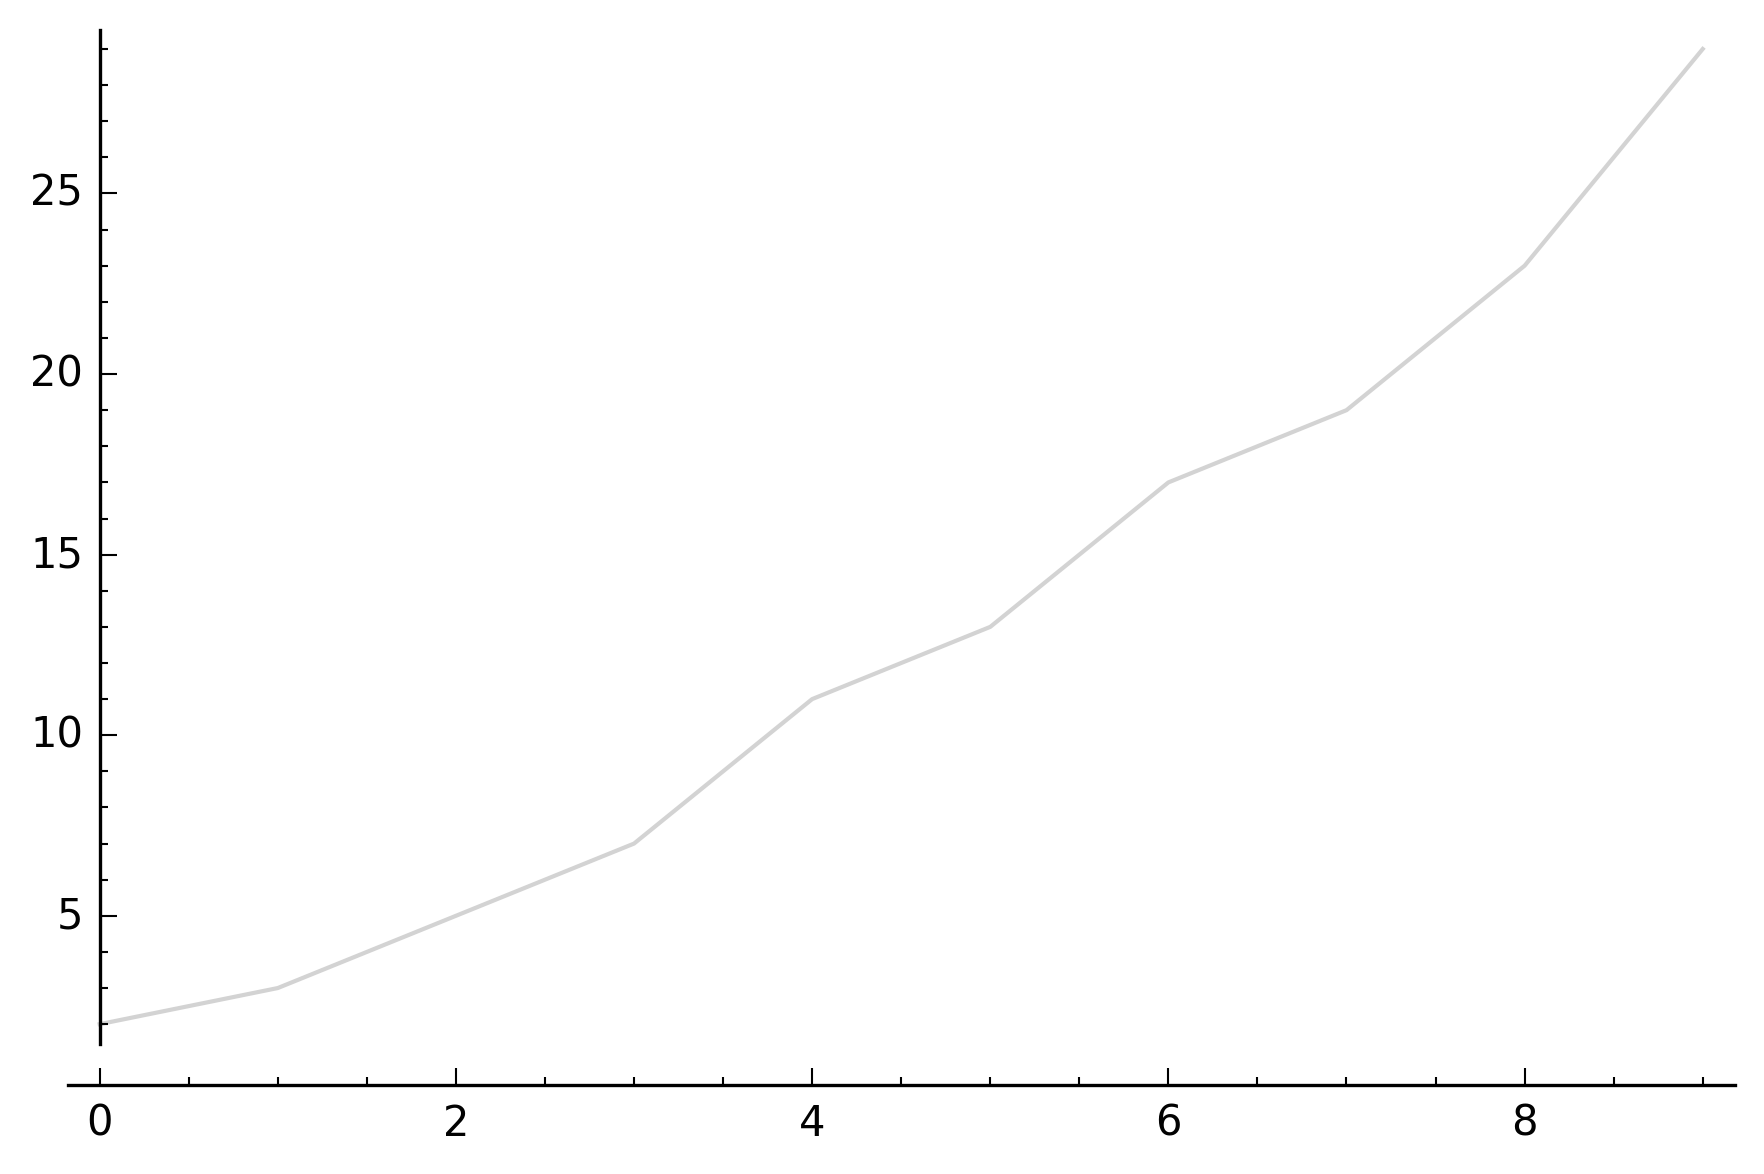
\includegraphics[width=0.6\textwidth]{line-plot-sage.png}
\end{center}

In vanilla Python, you can use matplotlib\footnote{\url{http://matplotlib.org}}

\lstset{language=sage,label= ,caption= ,captionpos=b,numbers=none}
\begin{lstlisting}
import matplotlib.pyplot as plt
X = range(10)
Y = [2, 3, 5, 7, 11, 13, 17, 19, 23, 29]
plt.plot(X, Y)
plt.ylabel('primes!!!')
plt.savefig("line-plot-matplotlib.png", dpi=300r, bbox_inches='tight')
plt.close()
\end{lstlisting}

\begin{center}
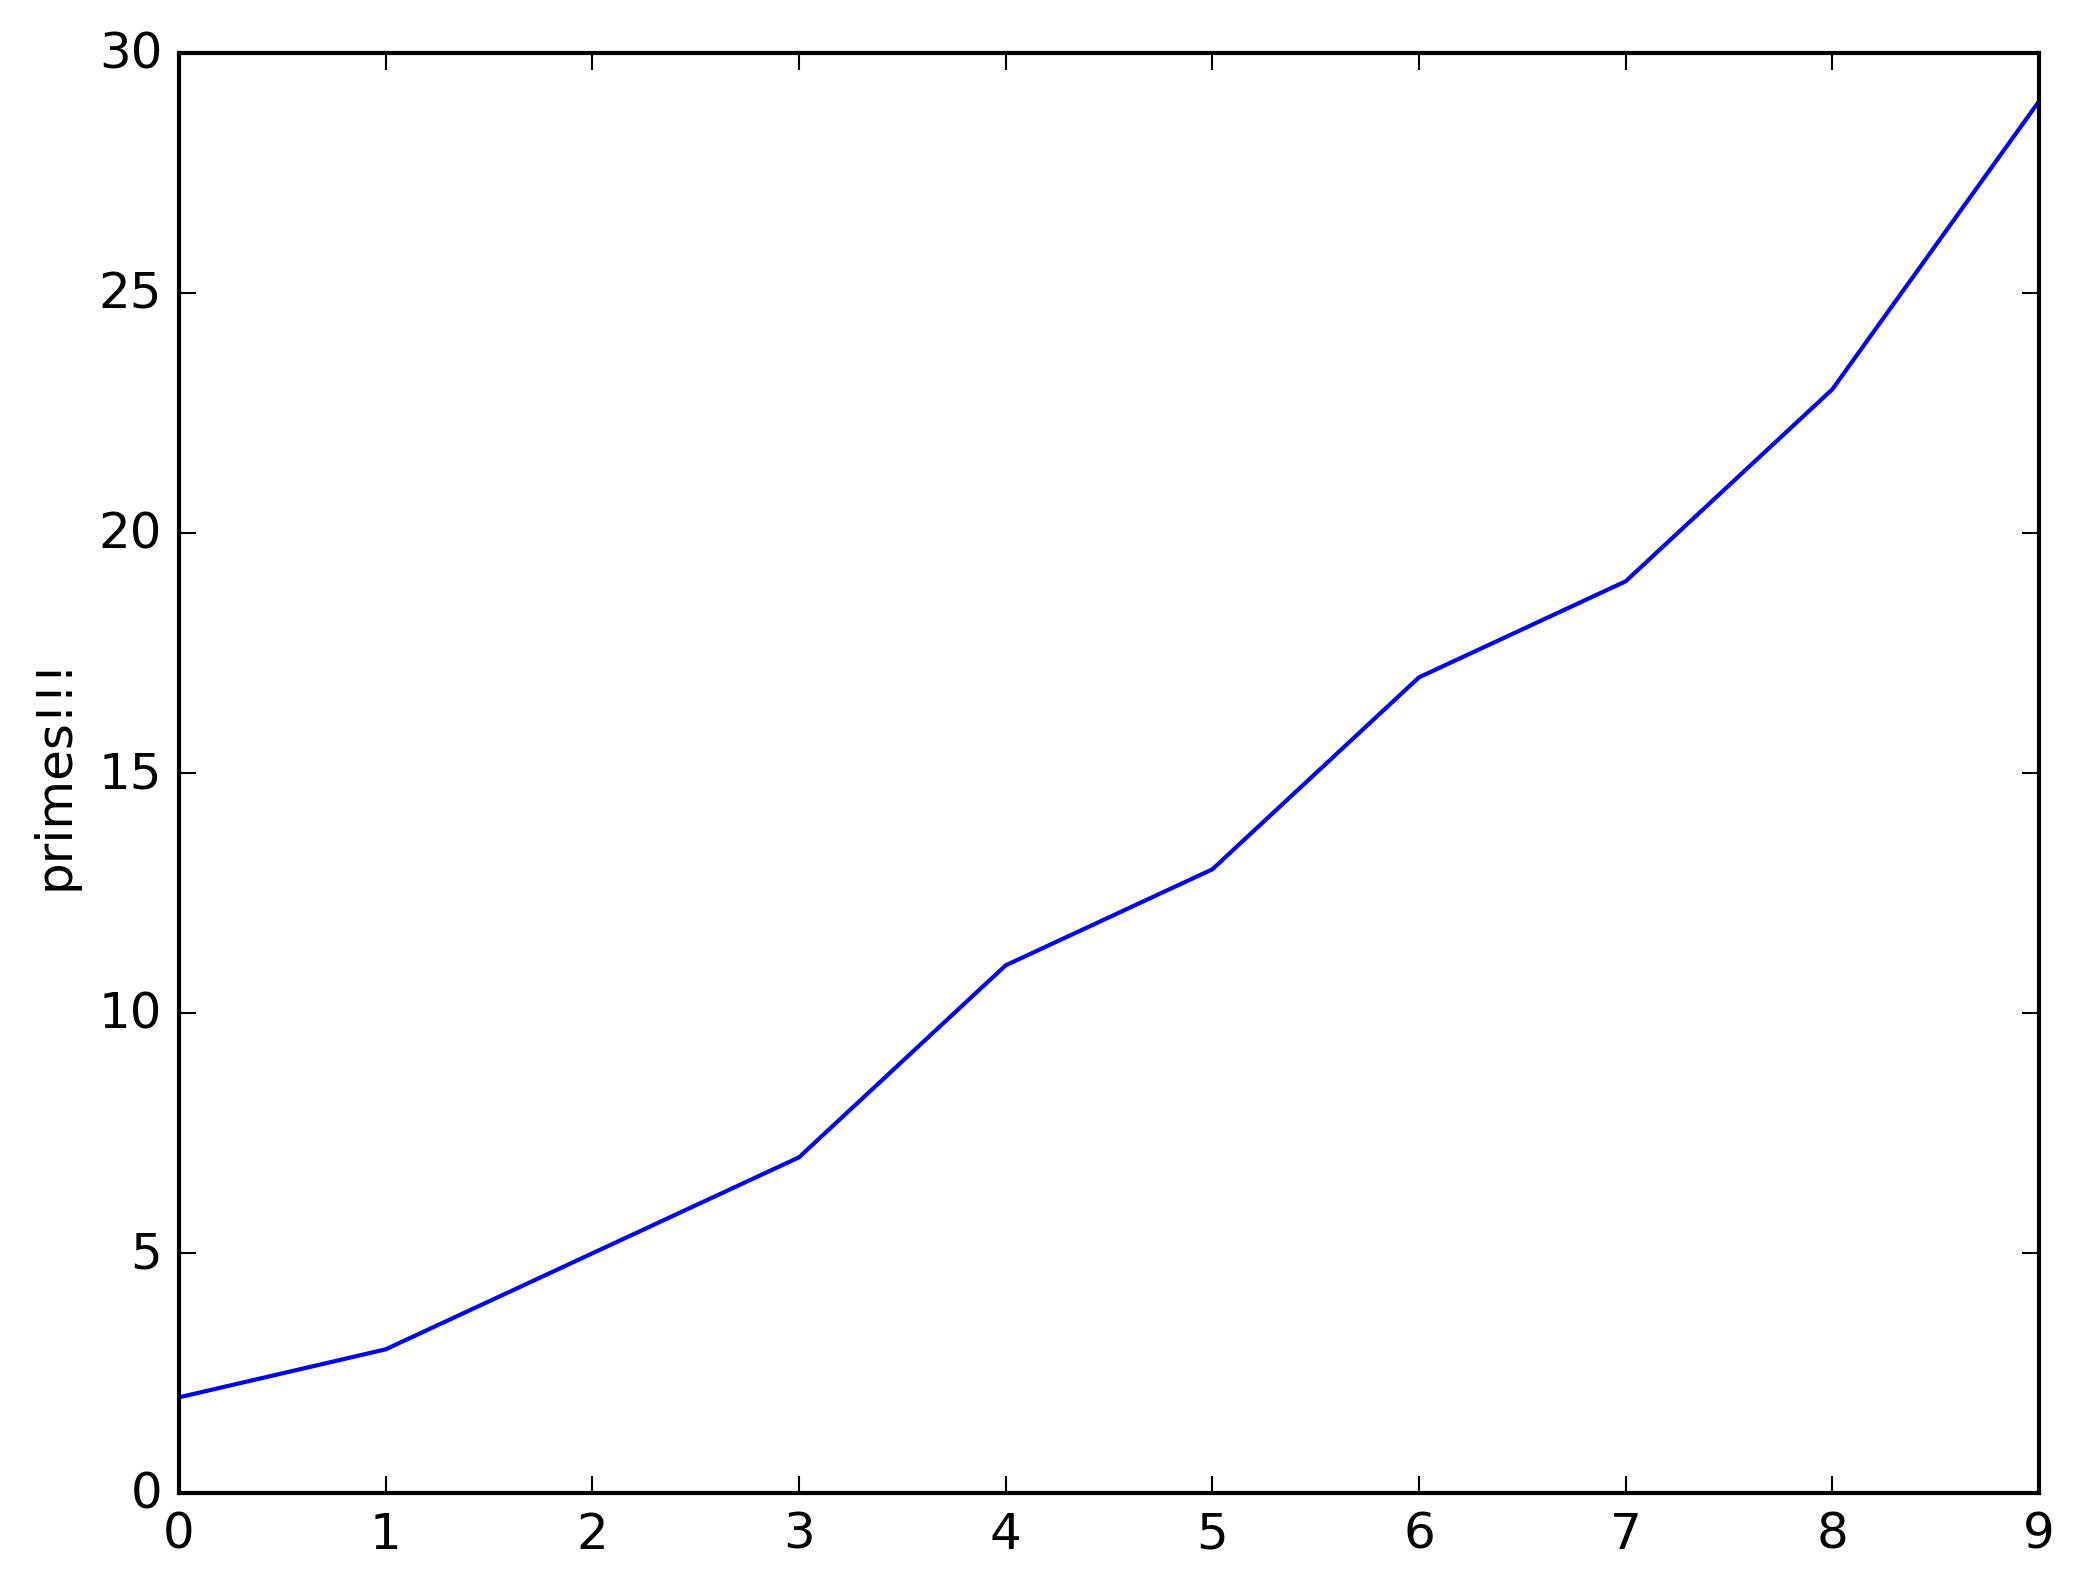
\includegraphics[width=0.7\textwidth]{./line-plot-matplotlib.png}
\end{center} 

\subsection{GSA}
\label{sec:org8ef7940}

Schnorr’s geometric series assumption (GSA) states that the norms of the Gram-Schmidt vectors after lattice reduction satisfy \[bla \] where \(n\) is the dimension of the lattice. Check how well this assumption holds for various block sizes of BKZ and BKZ 2.0.

\subsection{Costs}
\label{sec:org532b48b}

\begin{itemize}
\item Measure cost

\item Compare statistics
\end{itemize}

\section{3 — Dual Attack}
\label{sec:orgc4ccf27}

\begin{itemize}
\item Given a SIS instance, mount the best attack according to the model

\item (opt) Improve it using cleverer strategies (e.g. autotuned progressive strategy)
\end{itemize}

\section{4 — Primal Attack}
\label{sec:org0f652f8}

\section{5 — Pruned Enumeration}
\label{sec:org75a2cce}

Improve the previous by introducing a pruned enumeration on the whole lattice after BKZ reduction

\section{6 — Lattice Challenge}
\label{sec:org5d4995b}

\url{https://www.latticechallenge.org/lwe\_challenge/challenge.php}
\end{document}